% !TEX encoding = UTF-8
% !TEX TS-program = pdflatex
% !TEX root = ../tesi.tex

%**************************************************************
\chapter{Documentazione}
\label{cap:documentazione}
%**************************************************************
\intro{In questo capitolo si descrive la documentazione prodotta per l'applicativo sviluppato durante il periodo di stage.} 
	\section{Codice}
		Il codice prodotto durante il periodo di stage è stato scritto interamente per lo sviluppo dell'engine, che consiste in un unico progetto Maven. \\
		Per la sua documentazione, si è deciso di seguire lo standard JavaDoc, in questo modo si può generare un sito con la documentazione di tutte le classi/metodi prodotti tramite \texttt{mvn site}. \\
		Tutte le classi e i metodi son stati quindi preceduti da un commento descrivente l'invariante, le precondizioni, gli input e infine l'output aspettato da essi, con eccezione del controller principale dell'API, che è stato documentato tramite un file Swagger descritto nel capitolo successivo. 
	\section{Manuali}
		Lo stage richiedeva che al termine della codifica, fossero redatti i seguenti due manuali:
		\begin{itemize}
			\item Manuale Manutentore
			\item Manuale Installazione
		\end{itemize}
		Nel primo documento si ha affrontato la manutenzione del progetto: in esso infatti si è andato a descrivere come è stato creato il progetto, e come si intende esser sviluppato. Dentro si può trovare una descrizione dei package, una descrizione ad alto livello della logica dell'engine e infine i punti di estensione, quindi quelle parti del codice che probabilmente in un futuro si vorrà sapere come estendere per aggiungere funzionalità (nel caso di questo progetto, come aggiungere canali di notifica e come cambiare / aggiungere un provider diverso da Redmine)\\
		Nel secondo invece si vuole descrivere il processo di deploy dell'applicativo. In esso infatti si possono trovare i requisiti hardware minimi del server di deploy, le configurazioni e i servizi che tale server deve avere, e infine una guida su come far partire l'applicativo. In quanto il progetto richiedeva anche conoscenze esterne, come il saper creare un Bot Telegram, o come trovare un'ID di un gruppo Telegram, si è inserito inoltre una guida all'ottenimento di questi dati, oltre che all'utilizzo dei vari file XML necessari per il corretto funzionamento dell'engine.
	\section{API}
		Per quanto riguarda l'API, è stato prodotto un file Swagger descrivente input e output di ogni endpoint, così da poter generare PDF di documentazione esportabili, e avere una chiara visuale di come deve essere usata tale API.
		Il file redatto, se interpretato dal sito Swagger, genera la seguente documentazione:
		\begin{center}
			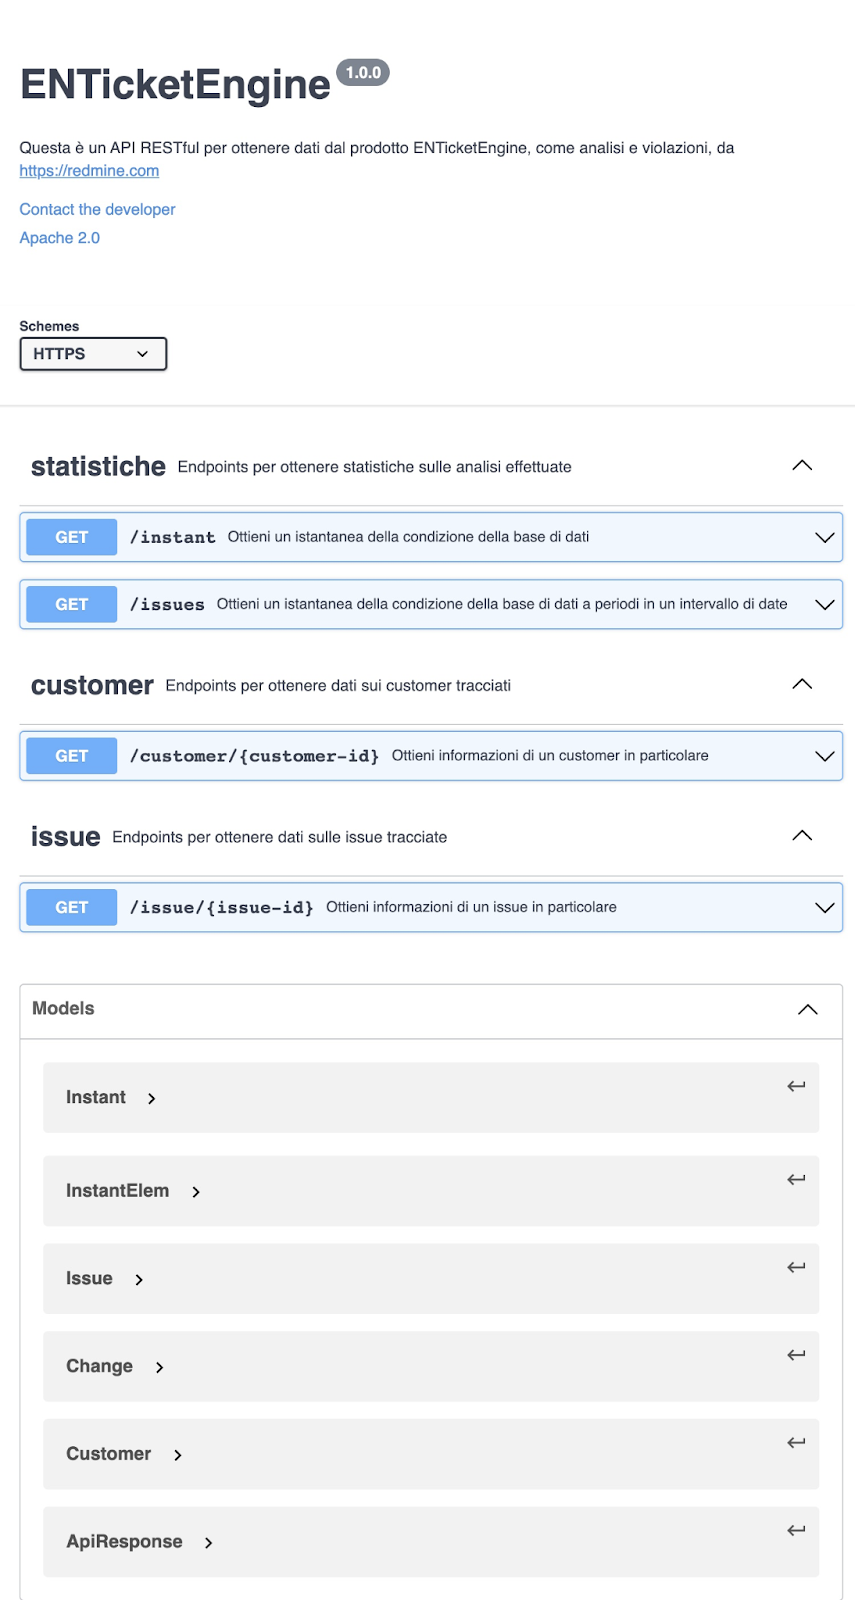
\includegraphics[keepaspectratio = true, height=20cm]{immagini/swagger.png}
			\captionof{figure}{File Swagger API}
		\end{center}